\chapter{Measurement of Directional Characteristics III}\label{ax:directional_3}
This appendix serves as a protocol to a series of measurements conducted between the 10\textsuperscript{th} and 12\textsuperscript{th} of May  2018 in the large anechoic chamber (B4-111) at the acoustic lab of Aalborg University at Fredrik Bajers Vej 7.\\
The goal of these measurements is investigating the behaviour of a loudspeaker array consisting of three of the loudspeakers that have been featured in \autoref{ax:directional_1} and \ref{ax:directional_2}.

\section*{Measuring Equipment and Materials}
The following measuring equipment was used:
\begin{itemize}[noitemsep]
\item Microphone \gls{bandk} 4144
\begin{itemize}[noitemsep]
\item AAU-number: 06552
\item Serial number: 297090
\end{itemize}
\item Preamplifier GRAS 26AK
\begin{itemize}[noitemsep]
\item AAU-number: 56526
\item Serial number: 32810
\end{itemize}
\item Power supply \gls{bandk} 2636
\begin{itemize}
\item AAU-number: 08022
\item Serial number: 
\end{itemize}
\item Calibrator \gls{bandk}\ 4231
\begin{itemize}[noitemsep]
\item AAU-number: 33691
\item Serial number: 2115338
\end{itemize}
\item 2 pcs. Power Amplifier Pioneer A-616
\begin{itemize}[noitemsep]
\item AAU-number: 08249, 08699
\item Serial number: HJ9404841S, JG9405804S
\end{itemize}
\item Sound card RME Fireface UCX
\begin{itemize}[noitemsep]
\item AAU-number: 108230
\item Serial number: 23811948
\end{itemize}
\item Turntable: Outline ET 250-3D
\begin{itemize}
\item Serial number: REIB0012
\end{itemize}
\item MATLAB r2017b on OSX 10.11.6
\item 3 pcs. Loudspeaker SEAS 33 F-WKA
\end{itemize}

The following material was used:
\begin{itemize}[noitemsep]
%\item \SI{1/2}{\inch} to \SI{1}{\inch} preamp adapter
\item Microphone clip
\item Microphone stand
\item LEMU cable
\item \gls{bandk} cable
\item XLR cables
\item Ethernet cable
\item miscellanious adapters
\item 3 pcs. Loudspeaker cabinet, plywood, outside dimensions: (400x400x400)\SI{}{\milli\meter}, wall~thickness:~\SI{20}{\milli\meter}, equipped with \citep{seas33}
\item Speaker mount for turntable
\begin{itemize}[noitemsep]
\item Steel mounting contraption, see \autoref{fig:speakerstand}
\item 3 speaker legs, \SI{40}{\milli\meter} box section, top: aluminium, {\(\varnothing\)~:~\SI{34.8}{\milli\meter}}, height: \SI{1}{\meter}
\item Circular \gls{mdf} cutout, thickness: \SI{12}{\milli\meter}, {\(\varnothing\)~:~\SI{800}{\milli\meter}}
\item \gls{mdf} cutout, thickness: \SI{20}{\milli\meter}, surface: approx. (300x600)\SI{}{\milli\meter}, bolt pattern drilled according to the bottom side of the ET 250-3D turntable
\item \gls{mdf} cutout for counterweight mounting, thickness: \SI{12}{\milli\meter}, surface : (400x400)\SI{}{\milli\meter}
\item triangular cutout (isosceles), thickness: \SI{12}{\milli\meter}, approximate outside dimensions base width x height: (970x600)\SI{}{\milli\meter}
\item 2 Electrovoice S-200 speakers as counterweight
\item Ratchet strap
\item 4 bolts M8x80, associated washers
\item 6 bolts M8x30, associated washers
\item 8 sinkhead bolts M8x40, associated nuts and washers
\item miscellaneous woodscrews

\end{itemize}
\end{itemize}


\begin{figure}[h]\label{fig:speakerstand}
  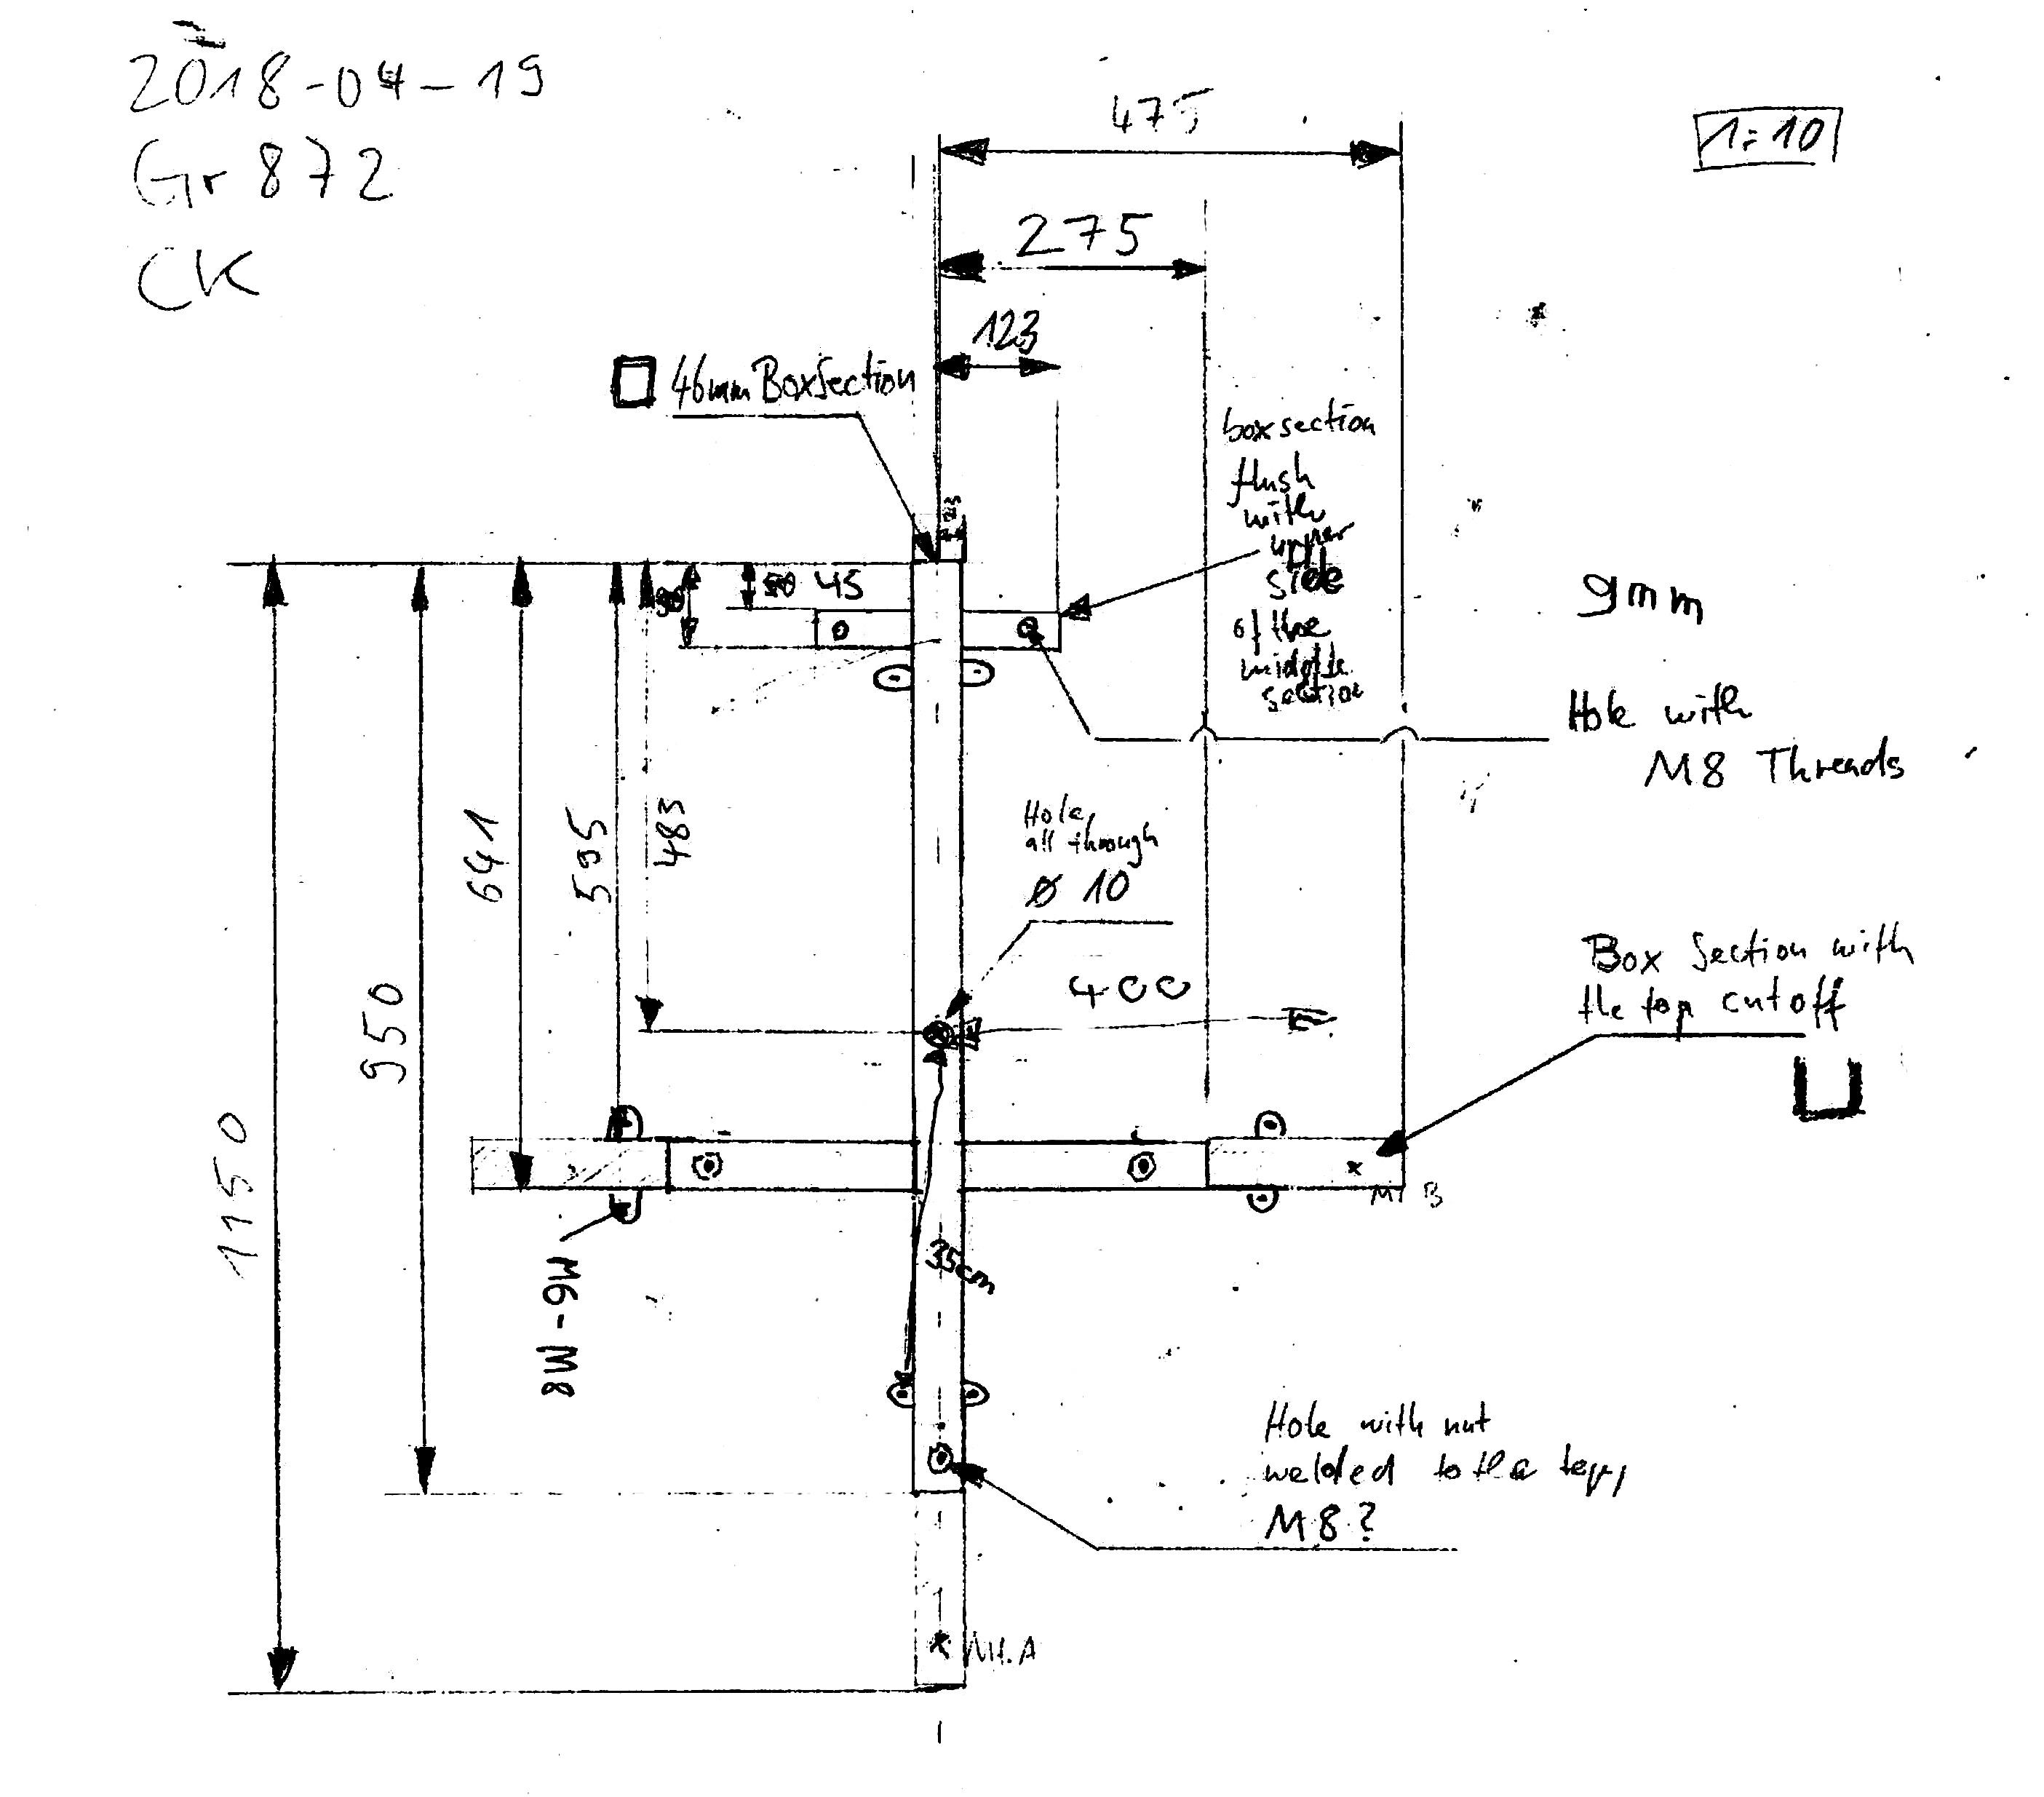
\includegraphics[width=\textwidth]{drawing_cut.jpg}
  \caption{Drawing of the base section of the array supporting contraption. It was used in combination with speaker legs with a length of $l\,=\,\SI{1}{\meter}$.}
\end{figure}
